\documentclass{report}
\usepackage{graphicx}

\author{Patrick Lindsay}
\title{Software Engineering Notes}

\newcommand*{\glossaryname}{Dictionary}
\usepackage[nonumberlist]{glossaries}
\newcommand{\define}[2]{%
 \newglossaryentry{#1}{name=#1, description={#2}}%
 \glslink{#1}{}%
}
\makeglossaries

\begin{document}
\maketitle
\tableofcontents
\newpage
\part{Notes}
\chapter{Software Life-Cycle Model}
	\section{Overview}
	\underline{Software Engineering} - The application of sound engineering practices to software creation and maintenance.
		\subsection{Software development Life Cycle (Traditional Approach)}
			\begin{itemize}
				\item Requirements Phase
				\item Analysis or Specification Phase
				\item Design Phase
				\item Implementation/Integration Phase
				\item Maintenance Phase
				\item Retirement
			\end{itemize}
		\subsubsection{Requirements Phase}
			\begin{itemize}
				\item Determining the \textsc{needs} and \textsc{wants} of the client or customer.
				\item Determining the constraints of the system.
			\end{itemize}
		\subsubsection{Analysis or Specification Phase}
			\begin{itemize}
				\item After analyzing the requirements, construct a \emph{specification document} which explicitly describes what the product is to do, and the constraints under which it must operate.
				\item This includes the description of the input, output, actions, and UI.
				\item The specification document can be used as part of a contract with the client.
			\end{itemize}
			\paragraph{Problems with the Spec Document}
			\begin{enumerate}
				\item Ambiguity - one sentence may have more than one interpretation.
				\item Incompleteness - relevant fact or requirement is left out.
				\item Contradiction - two places in the spec document are in conflict.
			\end{enumerate}
		\subsubsection{Design Phase}
			\begin{itemize}
				\item Construct an \emph{Architectural Design}.
				\item Construct a \emph{Detailed Design}.
				\item Test for \emph{traceability}.
			\end{itemize}
			\begin{enumerate}
				\item \underline{Architectural Design} - Description of the product in terms of modules.
				\item \underline{Detailed Design} - Description of each module.
				\item \underline{Traceability} - each part of the design can be traced to a statement in the specification document.
			\end{enumerate}
		\subsubsection{Implementation Phase}
			\begin{itemize}
				\item Code each module from the detailed design.
				\item Programmer tests his/her own code separately.
				\item Modules are combined and tested by developers.
				\item Product is tested by SQA group. This is called product testing.
				\item Project is given to the client for acceptance testing.
			\end{itemize}
		\subsubsection{Maintenance Phase}
			\begin{itemize}
				\item Corrective Maintenance - bug squashing
				\item Enhancement Maintenance - Updates
				\begin{itemize}
					\item Perfective - client makes new demands
					\item Adaptive - changes in the environment of the product requires changes in the software.
				\end{itemize}
				\item Perform regression testing - insuring that changes have not affected already working functionality.
			\end{itemize}
		\subsubsection{Retirement Phase}
			\begin{itemize}
				\item Determining if desired changes are too costly.
				\item Determining if a product is obsolete.
			\end{itemize}
	\subsection{Four Components of the Software Engineering Enterprise}
	The four P's
	\begin{enumerate}
		\item Process
		\item Project
		\item People
		\item Product
	\end{enumerate}
		\subsubsection{Process}
			\begin{itemize}
				\item The process is sometimes called the life-cycle model or development sequence.
				\begin{itemize}
					\item Waterfall
					\item Spiral
					\item Incremental Build
				\end{itemize}
				\item Makes use of several process frameworks.
				\begin{itemize}
					\item Personal Software Process (PSP)
					\item Team Software Process (TSP)
					\item Capability Maturity Model (CMM)
				\end{itemize}
				\item Documentation Standards
				\begin{itemize}
					\item IEEE
					\item ANSI
				\end{itemize}
			\end{itemize}
		\subsubsection{Project}
			\begin{itemize}
				\item The set of activities needed to produce the required product.
				\item Project management is extremely important.
				\item Many projects are not about developing new products, but maintaining already existing \emph{legacy} systems.
			\end{itemize}
		\subsubsection{People}
			\begin{itemize}
				\item Team Organization
				\item Team Management
				\item Relationship with customer or client
				\item Relationship with end users
				\item Communication with upper management
			\end{itemize}
		\subsubsection{Product}
			Includes
			\begin{itemize}
				\item Requirement Specification Document
				\item Design Document
				\item Source Code
				\item Executable
				\item User Manuals
			\end{itemize}
	\chapter{Traditional Software Engineering Process}
		\subsection{Historical Influences}
			\begin{itemize}
				\item Structured programming (Edsger Dijkstra's letter calling "GOTOs" harmful) uses sequence control, iteration, invoking functions
				\item Object Oriented paradigm: the use of objects with data and functionality which can represent real-world entities.
			\end{itemize}
			\textit{Note:\\Silver Bullet ca. 1980s\\ Likened the software crisis to a werewolf.  Object Oriented Paradigm was the Silver Bullet.\\It did not work as expected.}
			\begin{itemize}
				\item Design Patterns: stock of reusable design elements (templates)
			\end{itemize}
		\subsection{Component Reuse}
			A component as defined by Meyer is "a program element satisfying:"
			\begin{enumerate}
				\item The element may be used by other program elements. (Clients)
				\item The clients and their authors do not need to be known to the element's author
			\end{enumerate}
		\subsection{Key Expectations of Software Engineering}
			\begin{enumerate}
				\item Decide in advance what the specific quality measures are to be for the project and product.\\
					\textit{Predetermine quantitative quality goals.}
				\item Gather data on all projects to form a basis for estimating future projects.
				\item All requirements, designs, code and test materials should be freely and easily available to all members of the team.\\
					\textit{Source code should always be available to all team members in an easily accessible and interpreted way.\\
								Git, Mercurial, etc.}
				\item A process should be followed by all team members. \textit{Uniformity}
					\begin{enumerate}
						\item Design only against requirements.
						\item Program only against design.
						\item Test only against requirements and design.\\
						\textsc{Always follow the recipe!}
					\end{enumerate}
				\item Measure and achieve quality goals.
			\end{enumerate}
	\section{Methods}
		\emph{Be able to draw and discuss these.}
		\subsection{Waterfall Method}
			\textsc{See diagram 52.9 on pg 53.}
			\begin{itemize}
				\item First described by William\textit{(?)} Royce in 1970.
				\item No phase is complete until documentation for that phase has been completed and approved by the SQA group.\\
					\textit{Very orderly; heavy on documentation.}
				\item Has been used with great success on a variety of products.
				\item Feedback loops permits modifications to be made to the previous phase.
			\end{itemize}
			\subsubsection{Advantages}
				\begin{enumerate}
					\item Enforced disciplined approach
					\item Requirement that documentation be provided at each phase.
					\item All products of the phase must be checked by SQA.
					\item Inherent aspect of each phase is testing.
				\end{enumerate}
			\subsubsection{Disadvantages}
				\begin{itemize}
					\item The resulting specification document may not be able to be understood by the client.
					\item It can lead to the construction of product that does not meet the client's needs.					
				\end{itemize}
		\subsection{Rapid Prototype Model}
			\textsc{See diagram on pg 55.}
			Construction of a functional subset of the desired product in order to allow the client and the developer to interact.\\
			\textit{Keyword is rapid.  This is a thrown-together, proof-of-concept type project; a mock-up.}
			\subsubsection{Advantages}
				\begin{itemize}
					\item The process is linear and possibly faster than the Waterfall Model
					\item Increases interaction between client and developer.
				\end{itemize}
			\subsubsection{Disadvantages}
				\begin{itemize}
					\item Client may inaccurately think the product is almost complete when viewing the prototype.
					\item Developer may attempt to use the prototype as part of the final product.
				\end{itemize}
		\subsection{Waterfall-Rapid Prototype Hybrid}
			May form a hybrid model using the rapid prototype as the first phase in the Waterfall Model in order to increase interaction but allow for feedback loops within the development of the product.
		\subsection{Incremental Model}
			Software is implemented, integrated, and tested as a series of incremental builds.\\
				\textit{Code pieces providing specific functions.}
			\subsubsection{Advantages}
				\begin{enumerate}
					\item Results in builds which can be developed in weeks, not months or years.
					\item End user need not learn the entire product at one time.
					\item Client need not pay for the entire product at one time.
					\item Developer gets paid earlier.\\ (At each build delivery)
					\item Open-ended design makes maintenance easier.
					\item Easier to make changes during development.
				\end{enumerate}
			\subsubsection{Disadvantages}
				\begin{enumerate}
					\item Each new build must fit in without destroying existing builds.\\
						\textit{Regression Testing}
					\item Requires more careful to design to make it open to additions.
					\item Can degenerate to a build and fix product if broken into too few builds.
				\end{enumerate}
		\subsection{Spiral Model}
			\textsc{See Figure 2.12 on pg 63 and Figure 2.13 on pg 65.}
			\begin{itemize}
				\item A Waterfall Model with each phase preceded by risk analysis in an attempt to control or resolve risk.
				\item Each phase is 360º.
				\item The measure of the radius is the cumulative cost to date.
				\item The measure of the angle is the progress measure.\\
					\textit{Each phase is 360º.\\
								Requires a very experienced engineer.}
			\end{itemize}
			\subsubsection{Advantages}
				\begin{enumerate}
					\item The emphasis on alternatives and constraints supports the reuse of existing software.
					\item The incorporation of software quality as a specific objective.
					\item Answers the question of how much testing should be performed in terms of risks.
					\item Maintenance is simply another cycle of the spiral, the same as development.
				\end{enumerate}
			\subsubsection{Disadvantages}
				\begin{enumerate}
					\item Intended exclusively for internal development.\\
						\textit{Client and developer are members of the same organization.}
					\item \emph{Applicable only to large-scale projects.}
					\item Must have developers who are skilled at pinpointing the possible risks.
				\end{enumerate}
		\section{Agile Methods}
			\subsection{General}
				According to the Agile Manifesto, they value:
				\begin{itemize}
					\item Individuals and interactions over processes and tools.
					\item Working software over comprehensive documentation.
					\item Customer collaboration over contract negotiation.
					\item Responsiveness to change over following a plan.\\
						\textsc{You don't always have to follow the recipe!}
				\end{itemize}
				\subsubsection{Traits}
					\begin{itemize}
						\item Highly iterative
						\item Pair programming with a focus on teamwork and ego-less programming.\\
							\textsc{This is mandatory.}
						\item Early and planned testing.
						\item Story cards \textit{Similar to storyboards in movies.}
						\item Refactoring \textit{Turning working code into better code.}
						\item Feedback
					\end{itemize}
				\subsubsection{Principles Behind the Agile Manifesto}
					\begin{enumerate}
						\item Our highest priority is to satisfy the customer through early and continuous delivery of valuable software.
						\item Welcome changing requirements, even late in development. Agile processes harness change for the customer's competitive disadvantage.
						\item Deliver working software frequently, from a couple of weeks to a couple of months, with a preference to the shorter timescale.
						\item Business people and developers must work together daily throughout the project.
						\item Build projects around motivated individuals. Give them the environment and support they need and trust them to get the job done.
						\item The most efficient and effective method of conveying information to and within a development team is face-to-face conversation.
						\item Working software is the primary measure of progress.
						\item Agile processes promote sustainable development. The sponsors, developers, and users should be able to maintain a constant pace indefinitely.
						\item Continuous attention to technical excellence and good design enhances agility.
						\item Simplicity - the art of maximizing the amount of  work not done - is essential.
						\item The best architectures, requirements, and designs emerge from self-organizing teams.
						\item At regular intervals, the team reflects on how to become more effective, then tunes and adjusts its behavior accordingly.
					\end{enumerate}
			\subsection{Refactoring}
				\begin{itemize}
					\item Reduce software complexity
					\item Improve internal structure while preserving the behavior of the code.\\
						\textit{Prettifying}
					\item Improve software quality\\
						\textit{Readability, execution efficiency, size efficiency, etc.}
					\item Performed in response to "bad smells" in the code, undesirable characteristics\\
						\textit{Martin Fowler}
					\item Automated or manual\\
				\end{itemize}
	\chapter{Teams}
		\underline{Team} - a group of professionals organized in order to complete the task of creating a large software project.
		\section{Team Structure}
			\subsection{Project Factors Related to Structure of the Team}
				\begin{enumerate}
					\item Difficulty of the problem
					\item Size of the program in LOC or Function Points\\
						\textit{LOC stands for Lines of Code}
					\item Time the team will stay together
					\item Degree of modularity for program
					\item Required quality and reliability
					\item Rigidity of delivery date
					\item Degree of communication required
				\end{enumerate}
			\subsection{Jelled Team}
				\begin{itemize}
					\item A group of people which are so tightly knit that the attitude is that the whole is greater than the sum of the parts
					\item Egos are forgotten and the team becomes important
					\item Exhibits cohesiveness, team spirit, common definition of success
					\item Generally more productive, more motivated, and happier
				\end{itemize}
			\subsection{Why Don't All Teams Jell?}
				\begin{itemize}
					\item A frenzied work atmosphere
					\item High frustration causing friction among team members
					\item A "fragmented or poorly coordinated" software process
					\item An unclear definition on the team
					\item "Continuous and repeated exposure to failure" - M. Jackman \textit{Homeopathic Remedies for Team Toxicity}
				\end{itemize}
			\subsection{Necessary Team Traits}
				Personality
				\begin{itemize}
					\item Openness - intellectual curiosity
					\item Conscientiousness - self-discipline, pushing toward goals
					\item Extroversion - energy, emotions, seek company of others\\
						\textit{Being a people person}
					\item Agreeableness - compassionate and cooperative
					\item Neuroticism - how a person responds to stress, emotional stability
				\end{itemize}
			\subsection{How to Make Personality Traits Work}
				\begin{enumerate}
					\item Recognize people have different types of personalities
					\item Assemble a diverse team covering a range of personalities
					\item Create an open, honest, tolerant atmosphere in team meetings
				\end{enumerate}
		\section{Roles}
			\begin{itemize}
				\item \underline{Team Leader} - Responsible for overseeing all aspects of the team project; holds the tie-breaking vote.
				\item \underline{Technical Lead} - Expert on all technical aspects of the project, in particular the hardware and software used for development.
				\item \underline{Designer} - Designs the project and breaks the project into smaller pieces (\textit{Modules}) for the programmers.
				\item \underline{Lead Programmer} - Needs to have an understanding of the project as a whole; organizes all of the other programmers.
				\item \underline{Technical Writer} - Writes all documentation for the project (\textit{Team meeting minutes, Specification Document, Users' Manual})
				\item \underline{Configuration Management} - Maintains the code base for the project; could include CVS responsibilities.
				\item \underline{Quality Assurance} - Writes, maintains, and conducts all testing associated with the project.
			\end{itemize}
		\section{Organizational Structures}
			\begin{itemize}
				\item Democratic Team
				\item Hierarchical or Chief Programmer
				\item Team Manager/Team Leader
				\item Synchronize-and-Stabilize Team
				\item Agile Team
			\end{itemize}
			\subsection{Democratic Team}
				\begin{itemize}
					\item Group of up to 10 programmers
					\item Equal partnership with egoless programming
					\item Works well if the group is small, highly competent
					\item Problem with who is in charge
					\item Positive attitude about finding fault
					\item Good in research environment with difficult problem
				\end{itemize}
			\subsection{Hierarchical or Chief Programmer}
				\begin{itemize}
					\item One overall manager (\textit{Chief Programmer})
					\item Everyone understands the lines of authority\\
						\textit{One boss.}
					\item Team members tend to participate less in decisions; decisions are handed down from above
					\item May have a Programming Secretary and a Backup Programmer for the Chief Programmer
					\item Difficult to find one person adept at both managing and programming.
				\end{itemize}
			\subsection{Team Manager/Team Leader}
				\textit{See Figure 4.4, pg. 114}
				\begin{itemize}
					\item Split the responsibilities of Chief Programmer into Team Manager and Team Leader
					\item The Team Manager handles the nontechnical management
					\item The Team Leader deals with the technical issues of the project
					\item Results in programmers having two bosses
					\item May be difficult to determine if an issue is technical or nontechnical
				\end{itemize}
				\paragraph{Technical Organizational Structure for Large Projects}
					\begin{itemize}
						\item One Project Leader oversees several team leaders
						\item Each team leader has several programmers for which he/she is responsible
						\item Clear lines of communication\\
							\textit{Two level structure}
					\end{itemize}
			\subsection{Synchronize-and-Stabilize Team}
				\textit{Has been used by Microsoft}
				\begin{itemize}
					\item Small team led by a manager and having three to eight developers and three to eight testers working one-to-one with the developers
					\item Developers are given freedom to design and implement their portions as they wish
					\item Each day, the partial components are tested and debugged.
					\item Encourages creativity and innovation yet the daily synchronization keeps the project on track.
				\end{itemize}
			\subsection{Agile Team}
				\begin{itemize}
					\item Work in pairs (\textsc{Mandatory})
					\item Provide instant review
					\item Create test cases which are used for daily testing
					\item Remove the problem if one developer leaves, the knowledge does not disappear about a portion of the project
				\end{itemize}
	\chapter{Tools}
		\section{Tools for Software Engineers} 
			\begin{itemize}
				\item  Analytic (Theoretical) Tools:
					\begin{enumerate}
						\item  Stepwise Refinement
						\item Cost-Benefit Analysis
						\item Divide-and-Conquer
						\item Separation of Concerns
						\item Software Metrics
					\end{enumerate}
				\item Software Tools (CASE: Computer-Aided Software Engineering)
			\end{itemize}
			\subsection{Analytic Tools}
				\subsubsection{Stepwise Refinement}
					\begin{itemize}
						\item Process whereby a project is successively decomposed into more detailed instructions.
						\item In each step, a given task is written as a set of subtasks.
						\item Term was first coined by Niklaus Wirth in 1971.
						\item Helps to concentrate on relevant aspects of the current development phase and ignore details that need not be considered.
						\item A postponement of decisions on details until as late as possible.
						\item Critical to object-oriented paradigm.
					\end{itemize}
				\subsubsection{Cost-Benefit Analysis}
					\begin{itemize}
						\item Comparing estimated future benefits against future costs for a certain decision.
						\item Problems occur in that intangible benefits may be hard to quantify.
						\item May use past experience to project the estimates for benefits or costs.
					\end{itemize}
				\subsubsection{Divide-and-Conquer}
					\begin{itemize}
						\item Most agree this is the oldest analytical tool used in Software Engineering.
						\item Break a large problem into smaller subprograms that should be easier to solve.
						\item Idea used in the Unified Process.
						\item Good concept but no details on how to divide the problem
						\item \textit{Key difference from Stepwise Refinement is that Divide-and-Conquer does not necessarily procrastinate details.}
					\end{itemize}
				\subsubsection{Separation of Concerns}
					\begin{itemize}
						\item First introduced by Dijkstra in 1974.
						\item Process of breaking a software project into components which overlap as little as possible in relationship to functionality.
						\item Regression faults are minimized.\\
							\textit{If every component does one function (High Cohesion), making changes won't affect a lot of things.}
						\item Components are more reusable.
					\end{itemize}
				\subsubsection{Software Metrics}
					Measurements used to indicate:
					\begin{itemize}
						\item Size (LOC - Lines of Code)
						\item Duration (Months, years)
						\item Effort (Person-Months)
						\item Quality (Fault Density - Faults/1000LOC)
						\item Efficiency (Faults/Unit of time)
						\item Reliability (Mean time between failures)
					\end{itemize}
					Product/Process
			\subsection{CASE Tools}
				\begin{itemize}
					\item UpperCASE or front-end tools - used in the requirements, analysis and design workflows
					\item LowerCASE or back-end tools - used in the implementation and maintenance activities
				\end{itemize}
				\subsubsection{Types of CASE Tools}
					\begin{itemize}
						\item Data Dictionary - computerized list of all data defined within the product (type and location defined)\\
							\textit{Could be Upper or LowerCASE}
						\item Consistency Checker - tool which checks that everything in the design is in the specification document and everything in the specification document is in the design.
						\item Report Generator - tool which generates code needed for producing a report.
						\item Screen Generator - tool which generates the code necessary for a data capture screen.
						\item Structured Editor - a text editor which is designed to understand the structure of a program in a programming language, aiding in syntax fault prevention or early detection.
						\item Pretty Printer or Formatter - code often included with the structured editor which makes use of the language syntax structure to display the code in a standard manner (indenting, highlighting reserved words or comments)\\
							\textit{Try Sublime Text 2!}
						\item On-line Interface Checker - editor know every subprogram declared within the product and their parameter lists.
						\item Operating System Front End - tool which allows the programmer to give commands to the operating system from within the editor.
						\item Source Level Debugger \textit{LowerCASE}
						\item Interactive Source Level Debugger \textit{LowerCASE}
						\item Version Control Tool - keeps detailed record of each version of the project.\\
							\textit{Check out Git with GitHub or BitBucket!}
						\item Configuration Control Tool - manages multiple variations. \textit{LowerCASE}
					\end{itemize}
				\subsubsection{Grouped CASE Tools}
					\begin{itemize}
						\item CASE Workbench - collection of CASE tools that together support one or two activities.
						\item CASE Environment - collection of CASE tools which support the entire software process.
					\end{itemize}
		\section{Software Versions}
			\begin{itemize}
				\item During maintenance, at least two versions of the product will exist: the old version and the new version.
				\item \underline{Revision} - what we call the new version.
				\item \underline{Configuration} - the specific version of each artifact from which a given version of the complete product is built.
			\end{itemize}
	\chapter{Unified Process}
		\section{Phases of Unified Process}
			\subsection{Inception Phase}
				\begin{itemize}
					\item Determine whether it's worthwhile to develop the target product
					\item Determine economic viability
					\item Steps
						\begin{enumerate}
							\item Obtain domain knowledge
							\item Build business model\\
								\textit{Understand how the client operates within the domain.}
						\end{enumerate}
				\end{itemize}
				Questions to consider:
				\begin{enumerate}
					\item Is the proposed software cost effective?
					\item Can the proposed software be delivered on time?
					\item What risks are involved in developing the software and how can these risks be mitigated?
				\end{enumerate}
				Identify Risks
				\begin{enumerate}
					\item Technical risks
					\begin{itemize}
						\item Necessary experience?
						\item New hardware needed and will it be delivered on time?
						\item Software tools needed?
					\end{itemize}
					\item Not getting the requirements right
					\item Not getting the architecture (design) right
				\end{enumerate}
				\subsubsection{Documentation in the Inception Phase}
					\begin{itemize}
						\item Initial version of the domain model
						\item Initial version of the business model
							\textit{How the client operates in their domain.}
						\item Initial version of the requirements artifacts
						\item Preliminary version of the analysis artifacts
						\item Preliminary version of the architecture
						\item Initial list of risks
						\item Initial use cases
						\item Plan for elaboration phase
						\item Initial version of the business case\\
							\textit{Document that describes the cost-effectiveness of taking on the project}
					\end{itemize}
			\subsection{Elaboration Phase}
				\begin{itemize}
					\item The aim is to refine the requirements, refine the architecture, monitor the risks, refine the business case, and produce the software project management plan.
					\item Major activities are refinements of the previous phase.
				\end{itemize}
				\subsubsection{Elaboration Phase Deliverables}
					\begin{itemize}
						\item Completed domain model
						\item Completed business model
						\item Completed requirements artifact
						\item Completed analysis artifacts
						\item Updated version of the architecture
						\item Updated list of risks
						\item Software Project Management Plan (SPMP)
						\item Completed business case
					\end{itemize}
			\subsection{Construction Phase} 
				\begin{itemize}
					\item Aim is to produce the first operational-quality version of the product (beta release)
					\item Emphasis is on implementation and testing
					\item Components are coded and unit tested
					\item Components are combined (integrated) and tested again.
				\end{itemize}
				\subsubsection{Construction Phase Deliverables}
					\begin{itemize}
						\item Initial user manual and other manuals as needed
						\item All the artifacts of the beta release version
						\item Completed architecture
						\item Updated risk list
						\item Software Project Management Plan (SPMP)
						\item Updated business case if needed
					\end{itemize}
			\subsection{Transition Phase}
				\begin{itemize}
					\item Aim is to ensure that the client's requirements have been met
					\item Driven by feedback from the locations where the beta version is installed and tested
					\item Manuals are completed
					\item Faults are corrected
					\item Discover any unidentified risks
				\end{itemize}
				\subsubsection{Transition Phase Deliverables}
					\begin{itemize}
						\item All the artifacts of the final version
						\item Completed manuals
					\end{itemize}
					Refer to pg. 88 of the book.
	\chapter{Testing}
		\underline{Testing} - continual process carried on during the entire life cycle of software.\\
		\paragraph{V and V}
			\begin{itemize}
				\item Verification - determining whether a phase has been correctly carried out (at the end of the phase) 
				\item Validation - testing just before a product is delivered to the client to determine if it satisfies the specifications
			\end{itemize}
		\paragraph{Use of the Term Testing}
			We use the term testing instead of V and V because they imply that testing can wait until certain points in the process like the end of a phase, when testing must occur throughout the process.
			\subsection{Fault, Failure, Error, Defect}
				\begin{itemize}
					\item Fault - human mistake created in software
					\item Failure - observed incorrect behavior due to a fault
					\item Error - amount by which a result is incorrect 
					\item Defect - generic term used to encompass fault, failure, and error
				\end{itemize}
		\section{Software Quality}
			\begin{itemize}
				\item Extent to which the product satisfies its specifications
				\item Adherence to specifications
				\item Must be ensured at all times, not just added at the end of the product
				\item Every software developer must be personally responsible for the quality of their work.
			\end{itemize}
			\subsection{Software Quality Assurance}
				SQA group oversees the quality throughout the process
				\begin{itemize}
					\item Adherence to standards
					\item Correctness of each workflow
					\item Independent of the development team
				\end{itemize}
			\subsection{Categories of Testing}
				\begin{enumerate}
					\item Non-Execution-Based Testing (Reviews)
						\begin{itemize}
							\item Walkthroughs
								\begin{itemize}
									\item 4-6 person team  (Experience Senior Staff)
									\begin{itemize}
										\item Manager of the current workflow
										\item Member of the team on the current workflow
										\item Member of the team on the subsequent workflow
										\item Client Representative
										\item SQA group member
									\end{itemize}
									\item Material distributed to allow participants to prepare
									\item Each reviewer develops two lists: things they don't understand, things they think are incorrect
									\item Purpose is to find faults in a workflow or document such as the specification or the design document and create a list of faults for later correction
									\\\\
									Ways to conduct a walkthrough
									\begin{enumerate}
										\item Participant Driven - members present their lists to the team creating the document being tested which respond to each item (clarify questions, repair faults)
										\item Document Driven - chair walks the members through the document with stops at the unclear or possible faults
									\end{enumerate}
								\end{itemize}
							\item Inspections
								\begin{itemize}
									\item Proposed by Fagan in 1976 for testing designs and 
									\item Consists of five formal steps
									\item Conducted by team of size 4-5
										\begin{itemize}
											\item Moderator - both manager and leader of the inspection team
											\item Reader - leads team through the document
											\item Recorder - produces written report of detected faults
											\item Implementer/Tester
										\end{itemize}
									\item Steps:
										\begin{enumerate}
											\item Overview - presentation by one individual responsible for producing it after which given to participants
											\item Preparation - participants try to understand the document using lists of fault types and create checklist
											\item Inspection - one participant walks through using the checklists with the moderator creating a written report
											\item Rework - using the written report of faults, the individuals which created the document resolve the faults
											\item Follow-Up - moderator makes sure that everything in the report has been corrected or addressed and that no new faults were created in repairing the original faults
										\end{enumerate}
								\end{itemize}
						\end{itemize}
						\paragraph{Comparison of Walkthroughs and Inspections}
							\begin{itemize}
								\item Walkthroughs are 2 steps and inspections are more formal 5 steps 
								\item Inspections generally take longer but the extra time and effort spent can be cost effective
							\end{itemize}
					\item Execution-Based Testing
				\end{enumerate}
		\section{Reviews}
			\subsection{Strengths of Using Reviews}
				\begin{enumerate}
					\item Effective way to find faults in the specification document or the design document.
					\item Faults detected earlier in the process are less costly to repair or remove.
				\end{enumerate}
			\subsection{Metrics for Inspections}
				\begin{enumerate}
					\item Inspection Rate - the number of pages inspected per hour (for specifications and designs) or lines of code inspected per hour (for code inspection)
					\item Fault Density - number of faults per page or number of faults per KLOC
					\item Fault Detection Rate - number of major and minor faults detected per hour
					\item Fault Detection Efficiency - number of major and minor faults detected per person-hour
				\end{enumerate}
				These methods are used to determine whether the inspection process is working.
			\paragraph{Goals and Limits of testing}
				\begin{itemize}
					\item Goal: To maximize the number and severity of defects found per dollar spent
					\item Limit: Testing can only determine the presence of defects, never their absence. Correctness proofs are the only manner of proving the absence of defects.
				\end{itemize}
			\subsection{Levels of Testing}
				\begin{enumerate}
					\item Unit Testing - The earliest type of testing, testing the parts of the application (functions, modules, module combinations)
					\item Integration Testing - Validates the overall functionality of each stage
					\item Acceptance Testing - Validates the final product
				\end{enumerate}
			\subsection{Steps for Unit Testing}
				\begin{enumerate}
					\item Plan the general approach, resources, and schedule.
					\item Determine requirements-based characteristics to be tested.
					\item Refine the general plan.
					\item Design the set of tests.
					\item Implement the refined plan and design.
					\item Execute the test procedures.
					\item Check for termination.
				\end{enumerate}
			\subsection{Test Types}
				\begin{itemize}
					\item Black Box - Check correct output for given input as specified by the requirements
					\item White Box (or Clear Box) - Design test of cover all paths through the application.
					\item Gray Box - Consider limited details of the application with some of the Black Box techniques.
				\end{itemize}
				\subsubsection{Black Box Testing}
					\begin{itemize}
						\item Equivalence Partitioning - Division of the test input data into subsets
						\item Boundary Value Analysis - Testing for values which separate acceptable and unacceptable ranges.
					\end{itemize}
				\subsubsection{White Box Testing}
					\begin{itemize}
						\item Statement Coverage - Every statement should be executed by at least one test.
						\item Decision Coverage - Every branch of decision statements is executed.
					\end{itemize}
			\subsection{Planning Unit Tests}
				\begin{enumerate}
					\item Decide what the units are to be and who will test them.
					\item Decide how unit tests will be documented.
					\item Determine the extent of unit testing.
					\item Decide how and where to get the test input.
					\item Estimate the resources required.
					\item Arrange to track time, number, type, and source of defects.
				\end{enumerate}
			\subsection{Unit Testing of Methods}
				\begin{enumerate}
					\item Verify operation at normal parameter values.
					\item Verify operation at limit parameter values.
					\item Verify operation outside parameter values.
					\item Ensure that all instructions execute.
					\item Check all paths - both sides of branches.
					\item Check the use of all called objects.
					\item Verify the handling of all data structures.
					\item Verify the handling of all files.
					\item Check normal termination of all loops.
					\item Check abnormal termination of all loops.
					\item Check normal termination of all recursion.
					\item Check abnormal termination of all recursion.
					\item Verify the handling of all error conditions.
					\item Check timing and synchronization.
					\item Verify all hardware dependencies.
				\end{enumerate}
			\subsection{Class Testing}
				\begin{enumerate}
					\item Method Combination test
					\item Attribute-Oriented Test
					\item Testing Class Invariants
					\item State-based Tests
				\end{enumerate}
			\subsection{What is Tested During Execution Based Testing?}
				\begin{itemize}
					\item Utility - How useful it is or how it meets the needs of the user
					\item Reliability - Measuring the mean time between failures; reliable software rarely fails
					\item Robustness - valid output for valid input, error conditions handled correctly (satisfying the specifications)
					\item Performance - How well it meets the constraints
					\item Correctness - Valid output for valid input
				\end{itemize}
	\chapter{Modules and Objects}
		\section{Modules}
			Lexically contiguous sequence of statements bounded by boundary symbols, having an associated name.
			\paragraph{Cohesion and Coupling}
				\begin{itemize}
					\item \underline{Cohesion} - Measures of software quality relating to modules or classes.
					\item \underline{Coupling} - Measures used to quantify characteristics like reusability, reliability, etc.
				\end{itemize}
			\subsection{Cohesion}
				\begin{itemize}
					\item The degree of interaction within a module
					\item A description of the logical relationship between elements of a class
					\item The type of relationship that exists among the elements of each software entity.
				\end{itemize}
				\subsubsection{Types of Cohesion}
					\begin{enumerate}
						\item \underline{Coincidental} - No meaningful relationships among the elements of an entity. Difficult to describe the module's function(s)
						\item \underline{Logical} - Performs a series of related actions, one of which is selected by the calling module.
						\item \underline{Classical or Temporal} - Performs a series of actions related in time
						\item \underline{Procedural} - Performs a series of actions related by the sequence of steps to be followed by the product.
						\item \underline{Communicational} - Performs a series of actions related by the sequence of steps to be followed by the product performed on the same data.
						\item \underline{Informational} - Performs multiple functions, each with its own entry point, with independent code for each action, all performed on the same data structure.
						\item \underline{Functional} - Performs a single function or action.
					\end{enumerate}
					\textit{(Note: \#3-5 are sometimes called Flowchart Cohesion.)}
				\paragraph{Notes on Cohesion}
					\begin{itemize}
						\item As the cohesion number increases, so do the cohesion level and the desirability.
						\item Functional cohesion enhances reusability.
						\item Maintenance is easier to perform on a module with functional cohesion.
					\end{itemize}
			\subsection{Coupling}
				\begin{itemize}
					\item The degree of interaction between two modules.
					\item The type of relationship that exists between two software entities.
				\end{itemize}
				\subsubsection{Types of Coupling}
					\begin{enumerate}
						\item \underline{Content} - One software entity references the contents of another entity
						\item \underline{Common} - Software entities reference a shared global data structure
						\item \underline{External} - Software entities reference the same externally declared symbol
						\item \underline{Control} - One entity passes control elements as arguments to another entity
						\item \underline{Stamp} - A data structure is passed but not entirely used.
						\item \underline{Data} - One entity calls another and are not coupled as described above (every parameter passed is simple or a data structure entirely used)
					\end{enumerate}
			\subsection{Abstraction}
				\begin{enumerate}
					\item Data Abstraction
					\item Procedural Abstraction
				\end{enumerate}
				A means of achieving stepwise refinement by suppressing unnecessary details and accentuating relevant details.
			\subsection{Data Encapsulation}
				\begin{itemize}
					\item Data structure along with the actions or operations to be performed on that structure
					\item An example of abstraction
				\end{itemize}
				\subsubsection{Procedural Abstraction}
					Conceptualizing in terms of giving a name to a set of high-level actions which are specified by the body of the procedure.
				\subsubsection{Information Hiding}
					\begin{itemize}
						\item Better named "detail hiding"
						\item Concept introduced by Parnas
						\item Hiding the implementation details of a module from another using it
					\end{itemize}
				\subsubsection{Abstract Data Type (ADT)}
					\begin{itemize}
						\item Specification of a data type along with the operations on that type
						\item Supports both data and procedural abstraction
					\end{itemize}
				\subsubsection{Three Concepts Important to the OO Paradigm}
					\begin{enumerate}
						\item Inheritance*
						\item Polymorphism*
						\item Dynamic Binding
					\end{enumerate}
					\textit{* - These are especially important}
	\chapter{Reusability and Portability}
		\section{Reuse}
			\underline{Reuse} - Taking components of one product to be used in a different product with different functionality
			\subsection{Types of Reuse}
				\begin{enumerate}
					\item \textbf{Accidental} or \textbf{Opportunistic} Reuse - Developers realize that a component from a previously constructed product can be reused in the new project on which they are currently working.
					\item \textbf{Deliberate} or \textbf{Systematic} Reuse - Components are constructed with the purpose that they will be reused
				\end{enumerate}
				\subsubsection{Advantages of Deliberate Reuse}
					\begin{itemize}
						\item Components will be constructed with reuse in mind will be:
							\begin{itemize}
								\item more likely to be easier and safer to use.
								\item better documented.
								\item more thoroughly tested.
								\item adhere to a uniformity of style.
								\item more easily maintained.
							\end{itemize}
					\end{itemize}
				\subsubsection{Disadvantages of Deliberate Reuse}
					\begin{itemize}
						\item Can be expensive to the company
						\item Can be more time consuming
							\begin{itemize}
								\item Design
								\item Testing
								\item Documentation
							\end{itemize}
						\item May not be reused after time spent making it reusable
					\end{itemize}
			\subsection{Impediments to Reuse}
				\begin{enumerate}
					\item Ego
					\item Uncertainty of quality\\
						\textit{(Distrust of others' abilities)}
					\item Economic Reasons\\
						\textit{Afraid you might lose your job/Company won't need you anymore}
					\item Retrieval\\
						\textit{Can't find it}
					\item Expense\\
						\textit{To the company}
					\item Legality
					\item For COTS (\textit{Commercial Off-the-Shelf}) components - limited extensibility/modifiability
				\end{enumerate}
				May occur during design as well as implementation
			\subsection{Types of Design Reuse}
				\begin{enumerate}
					\item Company that develops software in one specific domain may set up repository of design components. (Library/Toolkit)
						\begin{enumerate}
							\item Tested module designs incorporated
							\item Reduce design time (and likely implementation)
							\item Increase design quality
						\end{enumerate}
					\item Application Frameworks
					\item Design Patterns
					\item Software Architecture
				\end{enumerate}
		\section{Design Patterns}
			\begin{itemize}
				\item Christopher Alexander - "Each pattern describes a problem which occurs over and over again in our environment, and then describes the core of the solution to that problem, in such a way that you can use this solution a million times over, without ever doing it the same way twice."
				\item Each design pattern is a solution to a general problem in the form of a set of interacting classes that have to be customized to create a specific design.
				\item Four Essential Elements
					\begin{enumerate}
						\item Pattern name
						\item Problem it solves
						\item Solution - elements making up the design
						\item Consequences - results and trade offs of applying	
					\end{enumerate}
			\end{itemize}
			\subsection{List of Design Patterns}
				\begin{enumerate}
					\item Abstract Factory
					\item Adapter
					\item Bridge
					\item Builder
					\item Chain of Responsibility
					\item Command
					\item Composite
					\item Decorator
					\item Façade
					\item Factory Method
					\item Flyweight
					\item Interpreter
					\item Iterator
					\item Mediator
					\item Memento
					\item Observer
					\item Prototype
					\item Proxy
					\item Singleton
					\item State
					\item Strategy
					\item Template Method
					\item Visitor
				\end{enumerate}
		\section{Portability}
			Software which is significantly easier to modify to run on another platform than it is to code from scratch.
			\subsection{Impediments to Portability}
				\begin{enumerate}
					\item Hardware Incompatibilities
					\item Operating System Incompatibilities
					\item Difference in numeric capabilities (\textit{32-bit v. 64-bit})
					\item Compiler Incompatibilities
					\item Data Formats
				\end{enumerate}
	\chapter{Planning and Estimating}
		\section{Cost}
			\subsection{Cost Estimation}
				Can occur at:
					\begin{itemize}
						\item Conceptualization Phase
						\item Requirements Analysis
						\item Design Phase
						\item Implementation Phase
						\item Implementation and Testing
					\end{itemize}
			\subsection{Cost Types}
				\begin{itemize}
					\item Internal Cost - cost to developer
						\begin{itemize}
							\item Salaries
							\item Hardware Support
							\item Software Support
						\end{itemize}
					\item External Cost - ???
				\end{itemize}
		\section{Size}
			\paragraph{Metrics for Size}
				\begin{enumerate}
					\item LOC - Lines of Code
					\item KDSI - Thousand Delivered Source Instructions
					\item Number of Operands and Operators
					\item FFP - Files, Flows, and Processes
					\item FP - Function Points
				\end{enumerate}
			\subsection{LOC and KDSI}
				\subsubsection{Problems With Using LOC or KDSI}
					\begin{enumerate}
						\item Creation of source code is only small part of total effort
						\item Same product in different languages would have different LOC
						\item Some languages have no concept of a line of code (LISP)
						\item Question as to whether only to count executable statements (omit declarations, comments, JCL (Job Control Language), reused code?)
						\item Not all code that is written is delivered
						\item Must wait until the project is finished to get the measurement
						\item Code generation tools
					\end{enumerate}
			\subsection{FFP}
				\begin{itemize}
					\item \underline{File} - collection of logically or physically related records, permanently resident in the product (transaction and temporary files do not count here)
					\item \underline{Flow} - data interface between the product and the environment (screen or report)
					\item \underline{Process} functionally defined logical or arithmetic manipulation of the data (sorting, validating, updating, etc.)
				\end{itemize}
			\subsection{FP}
				\underline{Function Points} - used to assess the size of a project
				\begin{enumerate}
					\item Identify the functions the application must have.
					\item For each function, compute:
						\begin{enumerate}
							\item External Inputs - EI
							\item External Outputs - EO
							\item External Inquiries - EIN
							\item Internal Logical Files - ILF
							\item External Logical Files - ELF
						\end{enumerate}
					\item Multiply the numbers from step 2 by specified values (see p. 274) This results in an unadjusted function point value (UFP).
					\item Compute the Technical Complexity Factor (TCF) using the effect of the 14 general characteristics of the project which have been assigned a value from 0-\textit{not present or no influence} to 5-\textit{strong influence throughout}. The 14 numbers are summed using the Total Degree of Influence (DI). Then the TCF is given by .65+.01*DI (see p.274)
					\item FP = UFP * TCF
				\end{enumerate}
				\subsubsection{Converting Function Points to Code}
					Once the function point value is computed, an estimate for the lines of code by multiplying by a constant associated with the language we plan to use for the application.
				\subsubsection{Techniques for Estimation of Size}
					\begin{itemize}
						\item Use comparisons with past jobs
						\item Use function point methods
							\begin{itemize}
								\item Compute unadjusted function points
								\item Apply adjustment process
							\end{itemize}
						\item Use LOC estimates to compute labor and duration using COCOMO formulas.
						\end{itemize}
			\subsection{COCOMO}
				\begin{itemize}
					\item Estimation method devised by Boehm in 1981
					\item COnstructive COst MOdel
					\item Depends on the LOC of a project
					\item 
				\end{itemize}
		\section{Cost Estimation Techniques}
			\begin{enumerate}
				\item Expert Judgment by Analogy - Consult a number of experts who have completed similar type projects.
				\item Bottom-up - Estimate each component from the leaf level and add, going upward in design.
				\item Algorithmic Cost Estimation - Use FF or FP and comu.
			\end{enumerate}
			\subsection{Software Project Management Plan}
				\begin{itemize}
					\item Plan which describes the proposed software development in full detail. (\textit{See p. 285})
					\item Consists of three main components:
					\begin{enumerate}
						\item The work to be completed
						\item The resources to be used to do the work
						\item Funding
					\end{enumerate}
				\end{itemize}
				\subsubsection{Work to be Completed}
					\begin{enumerate}
						\item Project function - work which continues throughout the project and is not related to any specific workflow.
						\item Activity - work which is related to a specific phase or workflow and has a definite beginning and end date
					\end{enumerate}
				\subsubsection{Resources}
					\begin{enumerate}
						\item People (varies during the duration of the project)
						\item Hardware
						\item Support Software (include CASE tools)
					\end{enumerate}
	\chapter{Requirements}
		\section{Requirements Analysis}
			\begin{itemize}
				\item Missed this. Get it from someone.
			\end{itemize}
			\subsection{Levels of Requirements Analysis}
				\begin{itemize}
					\item \underline{C-Requirements} - Documents what the customer wants and needs in a language clear to the customer (Customer Requirements)
					\item \underline{D-Requirements} - Documents the requirements in a specific, structured form (Developer Requirements)
				\end{itemize}
			\subsection{Why Write Requirements Documents?}
				Without such a document...
				\begin{enumerate}
					\item Team does not really know the goal it is trying to accomplish.
					\item Team cannot inspect its work properly
					\item Team cannot test its work properly
					\item Team cannot track its productivity
					\item Team cannot get adequate data on its practices
					\item Team cannot predict the size and effort of the next job
					\item Team cannot satisfy customer
				\end{enumerate}
			\subsection{Each Requirement Must Be...}
				\begin{itemize}
					\item Expressed properly
					\item Made easily accessible
					\item Numbered
					\item Accompanied by tests that verify it
					\item Provided for in the design
					\item Accounted for by code
					\item Tested in isolation
					\item Tested in concert with other requirements
					\item Validated by testing after the application has been built
				\end{itemize}
			\subsection{Requirements Analysis Process}
				\begin{enumerate}
					\item Identify the customer
					\item Interview customer representatives
						\begin{itemize}
							\item Identify wants and needs
							\item Exploit tools for expression
							\item Sketch GUI's
							\item Identify hardware
						\end{itemize}
					\item Write C-requirements (Review with customer)
					\item Inspect C-Requirements
					\item Build D-requirements (After customer approval)
				\end{enumerate}
		\section{Sources of Requirements}
			\begin{itemize}
				\item Customer Interviews
				\item Copies of currently used forms or software
				\item Customer site visit
				\item Surveillance cameras
				\item Rapid prototype
			\end{itemize}
		\section{Describing C-Requirements}
			\begin{enumerate}
				\item Use Cases
				\item Data Flow Diagrams
				\item State-Transition Diagrams
				\item Drafting User Interfaces (Rapid Prototype)
			\end{enumerate}
			\subsection{Use Cases}
				A concept invented by Jacobson used to express customer requirements in the form of interaction between an actor (type of user) and the application. It is identified by its name and by the type of user of the application (actor). Similar to a user story in Extreme Programming. \textit{See Pg. 318, Fig. 11.1}
			\subsection{Data Flow Diagrams}
				\begin{itemize}
					\item Requirements presented as the flow of data among processing elements
					\item Nodes represent processing units
					\item Arrows denote the flow of data
					\item Data stores are denoted by a pair of horizontal lines
					\item External agencies are represented as rectangles
				\end{itemize}
			\subsection{State-Transition Diagrams}
				\begin{itemize}
					\item Application exists as states or situations
					\item States are represented as nodes
					\item Transitions between states are represented with arrows
					\item Can also be used for a design tool
				\end{itemize}
			\subsection{Developing User Interfaces}
				\begin{enumerate}
					\item Know your user
						\begin{enumerate}
							\item Level of knowledge and experience
								\begin{enumerate}
									\item Computer literacy
									\item System experience
									\item Experience with similar applications
									\item Education
									\item Reading level
									\item Typing skill
								\end{enumerate}
							\item Physical characteristics
								\begin{enumerate}
									\item Age
									\item Gender
									\item Handedness
									\item Physical handicap
								\end{enumerate}
							\item Characteristics of user's tasks and jobs
								\begin{enumerate}
									\item Type of use (discretionary v. mandatory)
									\item Frequency of use
									\item Turnover rate for employees
									\item Importance of task
									\item Repetitiveness of task
									\item Training anticipated
									\item Job Category
								\end{enumerate}
							\item Psychological characteristics of user
								\begin{enumerate}
									\item Probable attitude toward job
									\item Motivation
									\item Cognitive style
										\begin{itemize}
											\item Verbal v. Spatial
											\item Analytic v. Intuitive
											\item Concrete v. Abstract
										\end{itemize}
								\end{enumerate}
						\end{enumerate}
					\item Understand the purpose of the user interface in terms of the application's overall purpose.
					\item Understand the principles of good screen design.
						\begin{enumerate}
							\item Consistency among screens
							\item Anticipate where the user will usually start
							\item Apply a hierarchy to emphasize the order of importance
							\item Apply principles of aesthetics
						\end{enumerate}
					\item Select the appropriate kind of window
						\begin{enumerate}
							\item Property window - display properties of an entity
							\item Dialog window - obtain information (Input)
							\item Message window - provide information (Output)
							\item Palette window - present a set of controls
							\item Pop-up window - amplify information
						\end{enumerate}
					\item Develop system menus
						\begin{enumerate}
							\item Provide a main menu (between 5 and 9)
							\item Display all relevant alternatives
							\item Match the menu structure to the structure of the application's tasks
						\end{enumerate}
					\item Select the appropriate device-based controls\\
						\textit{This refers to the physical means by which the user communicates their desires with the application (Joysticks, trackballs, graphics tablets, touch screens, mice, microphones, and keyboards.)}
					\item Select the appropriate screen-based controls\\
						\textit{Icons, buttons, text boxes, radio buttons\\
								Between 5 and 9, or organized into groups}
					\item Organize and lay out the window
					\item Choose appropriate colors
				\end{enumerate}
		\section{CASE Tools for Requirements}
			\begin{itemize}
				\item Graphical tool for drawing data flow diagrams
					\begin{itemize}
						\item + Easier to change a diagram stored in CASE tool than to redraw
						\item + Details of the product are stored in the CASE tool so the documentation is always available and updated
						\item - Not always user friendly
						\item - Almost impossible to program a computer to draw as pleasing a diagram as a human
					\end{itemize}
				\item Text Editor
				\item Survey construction tool
				\item Screen generator (For rapid prototyping)
			\end{itemize}
	\chapter{Writing the Specification Document} % (fold)	
		\section{Specification Document}
			\begin{itemize}
				\item Serves as contract between client and developer
				\item Must be clear and understandable by the client
				\item Must be complete and detailed for the design team
				\item Specifies exactly what the product is to do
				\item Describes the constraints of the system
				\item Describes acceptance criteria	Helps team select solution strategy
			\end{itemize}
			\subsection{Constraints} % (fold)
				\begin{enumerate}
					\item Timing
					\item Storage
					\item Security
					\item Response Time
					\item Portability
					\item Reliability
					\item Parallel Running
					\item Deadlines
				\end{enumerate}
			\subsection{Acceptance Criteria} % (fold)
				\begin{itemize}
					\item Set of series of tests which can be used to prove the product satisfies the specifications
					\item Indicates the developer's job is completed
					\item May be restatements of the constraints
				\end{itemize}
			\subsection{Solution Strategy}
				\begin{itemize}
					\item General approach to building the product
					\item Records are maintained of discarded strategies and why they were discarded. (This will help if the team must justify to SQA why they selected the method they did. It will also aid during maintenance.)
				\end{itemize}
		\section{Specification Document Writing Techniques}
			\begin{enumerate}
				\item Informal Methods
					\begin{itemize}
						\item Natural language, easy to learn
						\item Easy for client to understand
						\item Easy to incorporate ambiguities, contradictions
					\end{itemize}
				\item Semiformal Methods
					\begin{itemize}
						\item More precise than informal
						\item Client can understand
						\item Cannot handle timings
					\end{itemize}
				\item Formal Methods
					\begin{itemize}
						\item Most precise
						\item Reduce faults
						\item Support correctness proofs
						\item Difficult to learn
						\item Almost impossible for client to understand
					\end{itemize}
			\end{enumerate}
			\subsection{Semiformal Methods}
				\begin{enumerate}
					\item Data Flow Diagram (DFD) - Gane and Sarsen's graphical technique
					\item Problem Statement Language/Problem Statement Analyzer (PSL/PSA) - Computer aided technique
					\item Structured Analysis/Design Technique (SADT) - box and arrow diagramming language
					\item Software Requirements Engineering Model (SREM) - useful for specifying real-time systems and embedded systems
					\item Entity Relationship Modeling (ERM) - data oriented technique useful for specifying databases.
				\end{enumerate}
			\subsection{Formal Methods}
				Easier to validate and code
				\begin{enumerate}
					\item Finite State Machine (FSM)
					\item Petri Net - Carl Adam Petri in 1962
					\item Z \textit{/'zed/} - Formal specification language
					\item Anna - formal specification language for Ada
					\item Vienna Definition Language (VDL) - based on denotational semantics
				\end{enumerate}
				\subsubsection{Petri Net}
					\textit{See pg. 382}
					\begin{itemize}
						\item Useful for concurrent processes and synchronization
						\item Nondeterministic
						\item C = P, T, I, O
							\begin{itemize}
								\item P - Finite set of \textbf{places}	
								\item T - Finite set of \textbf{transitions}
								\item I - \textbf{Input} function mapping T to bags of places
								\item O - \textbf{Output} function mapping T to bags of places
							\end{itemize}
					\end{itemize}
				\subsubsection{Z}
					Four sections:
					\begin{itemize}
						\item Given sets (sets that need not be defined in detail), data types and constants
						\item State Definition\\
							\textit{Schema - group of variable declarations together with a list of predicates that constrain the possible values of the variables}
						\item Initial State - description of the system when first turned on
						\item Operations
					\end{itemize}
					\paragraph{Analysis of Z}
						\begin{itemize}
							\item Easy to find faults in specification written in Z
							\item Requires writer to be concise
							\item Allows for proofs
							\item Not too difficult to learn
							\item Has decreased the cost of software development
							\item Easy to translate into natural language for the client
						\end{itemize}
		\section{Testing during Specification Phase}
			\begin{itemize}
				\item Walkthroughs
				\item Inspections
				\item Correctness proofs
			\end{itemize}
		\section{CASE Tools}
			\begin{itemize}
				\item Graphical drawing tool for DFD or Petri Nets
				\item Data dictionary
				\item Combined drawing tool and data dictionary (And possibly a consistency checker)
					\begin{itemize}
						\item Analyst/Designer
						\item Software through pictures
						\item System Architect
					\end{itemize}
			\end{itemize}
		\section{Metrics}
			\begin{itemize}
				\item Size - number of pages in the document
				\item Quality - measure the number of faults of each type found during inspection
				\item Effort - counts of files, data items, and operations
			\end{itemize}
	\chapter{Design}
		\section{Implementation}
			\begin{itemize}
				\item The process of translating the detailed design into code.
				\item Unit implementation refers to coding the smallest part of the project which can be separately maintained.
			\end{itemize}
			\subsection{Selection of a Programming Language}
				\begin{enumerate}
					\item Client Requests
					\item ONly one available on the hardware
					\item Most Suitable
						\begin{itemize}
							\item For the application
							\item For the environment
							\item For the cost
						\end{itemize}
				\end{enumerate}
			\subsection{Goals of Implementation}
				\begin{enumerate}
					\item Satisfy the requirements specified in the detailed design.
					\item Conform to standards
					\item Document work
					\item Maintain records of time, defects
					\item Promote maintainability
				\end{enumerate}
			\subsection{Steps for Implementation}
				\begin{enumerate}
					\item Plan the structure of the code (complete detailed design)
					\item Self inspect the design or structure
					\item Type in the code complying to standards
					\item Self inspect your code
					\item Compile
				\end{enumerate}
			\subsection{Principles of Sound Implementation}
				\begin{enumerate}
					\item Try to reuse already existing code if possible.
					\item Enforce intentions (Code not to be used anywhere else in the application or to be used in other parts?)
					\item Use qualifiers like final, const, and abstract to enforce intentions
						\begin{enumerate}
							\item Final classes can't have descendants
							\item Final methods can't be overridden in inherited classes
							\item The value of final variables can't be changed
						\end{enumerate}
					\item Make members inaccessible if they are not specifically intended to be accessed directly
						\begin{enumerate}
							\item Make attributes private. Access through public accessors
							\item Make methods private if they are for use only by methods of the same class.
						\end{enumerate}
					\item Include examples in documentation
					\item List methods alphabetically rather than trying to find a calling order among them. (You may group private, protected, and public methods.)
				\end{enumerate}
		\section{Programming Practices}
			\subsection{Sound Programming Practices}
				\begin{enumerate}
					\item Use consistent and meaningful variable names
					\item Use prologue comments for each function giving input, actions, output, author and date, modification and date, files accessed, date tested and approved by
					\item Use no more than one statement per line
					\item Make good use of white space
					\item Restrict levels of nesting to three or four
					\item Be consistent with indenting
					\item Read in parameters instead of hard-coding constants
				\end{enumerate}
			\subsection{Hints for Working with Pointers}
				\begin{itemize}
					\item Avoid using pointer parameters in C++, use references instead.
					\item Never return a pointer to a new heap reference in C++.
					\item Collect your garbage
				\end{itemize}
			\subsection{Hints for Working with Functions}
				\begin{itemize}
					\item Avoid type inquiry. Use virtual functions instead.
					\item Avoid C++ friend functions except when obviously beneficial.
					\item Be careful overloading operators.
				\end{itemize}
			\subsection{Hints on Working with Exceptions}
				\begin{itemize}
					\item Catch only those exceptions you know how to handle.
					\item If the present method cannot handle the exception, there has to be a handler in an outer scope that can do so.
					\item If you can handle part of the exception, then handle and rethrow the exception for handling in the outer scope
				\end{itemize}
			\subsection{Hints on Error Handling}
				\begin{enumerate}
					\item Follow agreed-upon development process; inspect
					\item Consider introducing classes to encapsulate legal parameter values.
					\item Where error handling is specified by requirements, implement
					\item For applications that must never crash, anticipate all possible implementation defects (use defaults)
					\item Follow a consistent policy for checking parameters
				\end{enumerate}
		\section{Programming Standards}
		    \subsection{Examples of Programming Standards}
		    	\begin{enumerate}
		    		\item Naming Conventions
			    		\begin{enumerate}
			    			\item Name with concatenated words
			    			\item Begin class names with capitals
			    			\item Begin variables with lowercase letters
			    		\end{enumerate}
			    	\item Documentation for Methods
			    		\begin{enumerate}
			    			\item Preconditions
			    			\item Postconditions
			    			\item What the method does
			    			\item What parameters must be passed
			    			\item What exceptions it throws
			    			\item Reason for choice of visibility
			    			\item Ways in which instance variables are changed
			    			\item Known bugs
			    			\item Test description
			    			\item HIstory of changes
			    		\end{enumerate}
			    	\item Within Methods
			    		\begin{enumerate}
			    			\item Perform only one operation per line.
			    			\item Try to keep the size to one screen.
			    			\item Use parentheses within expressions even if they are not needed by the syntax.
			    		\end{enumerate}
			    	\item Documenting Attributes
			    		\begin{enumerate}
			    			\item Provide all application invariants
			    			\item State its purpose
			    		\end{enumerate}
		    	\end{enumerate}
		\section{Tools and Environments for Programming}
			\begin{itemize}
				\item IDE (interactive Development Environment) - used for allowing programmers to produce more code in less time
				\item Drag-and-Drop facilities for forming GUI components
				\item Graphical representation of directories
				\item Debuggers
				\item Wizards
			\end{itemize}
		\section{Defect Severity Classification}
			\begin{itemize}
				\item Major - Requirements not satisfied
				\item Medium - Neither major nor trivial
				\item Trivial - a defect that will not affect operation or maintenance, but just feels a little "meh"
			\end{itemize}
		\section{Integration}
			\subsection{Terms}
			    \begin{itemize}
			    	\item Iteration - a coherent stage of construction
			    	\item Build - one of sever carefully planned activities within an iteration
			    \end{itemize}
			\subsection{Roadmap for Integration}
				\begin{enumerate}
					\item Decode on the extent of all tests.
					\item For each iteration:
						\begin{itemize}
							\item For each build
								\begin{enumerate}
									\item Perform regression testing prior to build
									\item Retest functions if necessary
									\item Retest modules if necessary
									\item Test interfaces if required
									\item Perform build integration tests
								\end{enumerate}
							\item Perform iteration system and usability test
						\end{itemize}
					\item Perform installation tests
					\item Perform acceptance tests
				\end{enumerate}
		\section{Testing}
		    \begin{enumerate}
		    	\item Integration testing
		    	\item Interface testing
		    	\item System testing
		    	\item Usability testing
		    	\item Regression testing
		    	\item Acceptance testing
		    	\item Installation testing
		    \end{enumerate}
			\subsection{Integration Testing}
				\begin{enumerate}
					\item Decide how and where to store, reuse and code the integration test
					\item Execute as many unit tests as time allows
					\item Exercise regression testing
					\item Ensure build requirements are properly specified
					\item Exercise use cases that the build should implement (Test against the SRS)
					\item Execute the system tests supported by this build
				\end{enumerate}
				\subsubsection{Artifacts Involved in Integration Testing}
					\begin{enumerate}
						\item Use case model - set of use cases describing the typical usage of the application and sequence diagrams
						\item Test cases
						\item Test procedures
						\item Test evaluation
						\item Test plan
						\item Test components - source code for tests
						\item Defects - report on defects discovered, classified
					\end{enumerate}
			\subsection{Interface Testing}
				\textit{Get this bullet from someone.}
			\subsection{System Testing}
				\begin{itemize}
					\item Black box which validate the entire application against the requirements
					\item \textit{Messed this line up. Get it from someone.}
					\item \textit{Messed this line up. Get it from someone.}
				\end{itemize}
				\subsubsection{Types of System Testing}
					\begin{enumerate}
						\item Reliability/Availability (MTBF)
						\item Volume (large amounts of input)
						\item Usability
						\item Performance
						\item Configuration
						\item Compatibility
						\item Security
						\item Resource usage
						\item Installability
						\item Recoverability
						\item Serviceablity
					\end{enumerate}
				\subsubsection{Usability Testing}
					\paragraph{Attributes for Usability Testing} 
						\begin{enumerate}
							\item Accessibility - ease of navigation
							\item Responsiveness - average time taken to accomplish specified goals
							\item Efficiency - how minimal are the require steps to selected functionality
							\item Comprehensibility - how easy to understand and use with documentation and help
						\end{enumerate}
			\subsection{Regression Testing}
				Verifying that a project continues to pass the same designated set of system tests that it passed before a change was made.
			\subsection{Acceptance Testing}
				\begin{itemize}
					\item Designed to assure the customer that the project agreed upon has, in fact, been built.
					\item Witnessed officially by a customer representative
					\item May be the same as some of the system tests
				\end{itemize}
			\subsection{Installation Testing}
				\begin{itemize}
					\item Testing the application in the actual target hardware organization where it will be executing
					\item Perform the same system tests used during integration
				\end{itemize}
		\section{Test Documentation Standard}
		    \begin{enumerate}
		    	\item Introduction
		    	\item Test plan - items, scope, approach, resources, schedule, personnel
		    	\item Test design - items, approach and plan in detail
		    	\item Test cases
		    	\item Test procedures - steps for setting up and executing the test cases
		    	\item Test item transmittal report - item under test, physical location of results, person responsible for testing
		    	\item Test log - chronological record, physical location of test, tester name
		    	\item Test incident report - record of an event during testing requiring further investigation
		    	\item Test summary report
		    \end{enumerate}
		\section{Transition Iterations}
		    \begin{itemize}
		    	\item Find defects through customer use
		    	\item Test user documentation and help
		    	\item Determine realistically whether application meets requirements
		    	\item Retire deployment risks
		    	\item Satisfy miscellaneous marketing goals
		    \end{itemize}
		\section{Alpha Release}
		    \begin{itemize}
		    	\item After integration, project is given to in-house users for early prerelease use
		    	\item Purpose to provide feeback, defect information and advanced knowledge of the product
		    \end{itemize}
		\section{Beta Release}
			\begin{itemize}
		    	\item After integration - project is given to a part of the customer community with the understanding that they report defects found.
		    	\item Used to convince customers that there really is a product behind the vendor's promises.
		    \end{itemize}
	\chapter{Post-Delivery Maintenance}
		\paragraph{Why is Post-Delivery Maintenance Necessary?}
			\begin{enumerate}
				\item Corrective Maintenance - correcting a fault
				\item Perfective Maintenance - improving the effectiveness of the product
			\end{enumerate}
		\section{Facts About Post-Delivery Maintenance} 
			\begin{enumerate}
				\item More time spent on post-delivery maintenance than any other activity
				\item Approximately 67\% of the product cost
				\item The most challenging of all aspects of software production
				\item Incorporates aspects of all of the other workflows of the product.
				\item The most thankless development task
			\end{enumerate}
		\section{Problems with Post-Delivery Maintenance}
			\begin{enumerate}
				\item Product may have not been developed with maintenance in mind.
				\item Not considered glamorous
				\item Task often given to beginners, not the more experienced programmers
				\item Must avoid creating more faults when correcting one
			\end{enumerate}
		\section{Requirements for Post-Delivery Maintenance Programmers}
		    \begin{enumerate}
		    	\item Ability to locate the cause of a fault
		    	\item Ability to function without good documentation
		    	\item Ability to maintain documentation of changes
		    	\item Ability to perform regression testing
		    	\item Ability to perform requirements analysis, design and implementation for adaptive or perfective maintenance
		    	\item Ability to design tests for new functionality added
		    \end{enumerate}
		\section{Management of Post-Delivery Maintenance}
		    \begin{enumerate}
		    	\item Defect report filed by user
		    	\item Reports may be prioritized
		    	\item Work given to programmer for repair
		    	\item Results tested by SQA and documented
		    	\item Make sure changes do not adversely affect further maintenance
		    	\item Encourage client to avoid the moving target problem
		    \end{enumerate}
		\section{Special Problems with Object-Oriented Maintenance}
			\begin{enumerate}
				\item to understand an object, maintainer must understand the object's hierarchy
				\item \textit{Get bullet from someone.}
				\item \textit{Get bullet from someone.}
			\end{enumerate}
		\section{Reverse Engineering}
		    \begin{itemize}
		    	\item The process of recreating the design document and possible the SRS document, given the source code.
		    	\item Its need is due to the amount of legacy code in the industry
		    \end{itemize}
		\section{CASE Tools for Maintenance}
		    \begin{enumerate}
		    	\item Version Control
		    	\item Configuration Control Tool
		    	\item Pretty Printer
		    	\item Graphic tools
		    	\item Display class hierarchy
		    	\item Defect-tracking tool (Bugzilla)
		    \end{enumerate}
	\chapter{Detecting Obsolescence}
		\begin{itemize}
			\item \underline{Obsolescence} - the state of being which occurs when an object, service, or practice is no longer wanted even though it may still be in good working order.
		\end{itemize}
		\section{Areas to Consider}
			A solution may be obsolete if...
		    \begin{itemize}
		    	\item Your system can't handle increased workloads or the way you do business has changed.
		    	\item An organization adds headcount instead of reinvesting in technology
		    	\item The software engineers from your last project are no longer available
		    	\item Your reporting is less than stellar
		    	\item The solution doesn't allow you to get back to business quickly
		    	\item Your organization is witnessing larger-than-normal turnover or if delivering exceptional customer care is becoming a challenge
		    \end{itemize}
		\section{Causes of Software Obsolescence}
		    \begin{enumerate}
		    	\item Functional Obsolescence
		    	\item Technological Obsolescence
		    	\item Logistical Obsolescence
		    \end{enumerate}
		    \subsection{Functional Obsolescence}
		    	\begin{itemize}
		    		\item The software does not perform in the manner for which it was created
		    		\item May be cause by hardware changes, requirement changes or other software changes in a larger system
		    	\end{itemize}
		    \subsection{Technological Obsolescence}
		    	\begin{itemize}
		    		\item Inability to renew licensing agreements
		    		\item Software maintenance (support) terminates
		    		\item The original supplier no longer markets and sells the software
		    		\item More advanced software available
		    		\item Software written in obsolete, outdated, or inefficient language
		    	\end{itemize}
		    \subsection{Logistical Obsolescence}
		    	\begin{itemize}
		    		\item Digital media obsolescence
		    		\item Formatting changes
		    	\end{itemize}
		\section{How to Measure Obsolescence}
			\begin{enumerate}
				\item Physical Inspection of the code for inefficient layout, structural deficiencies, excessive or deficient capacities
				\item Comparative Analysis of existing software with a newer version of itself (if available)
			\end{enumerate}
		\section{Cost of Management of Software Obsolescence}
		    \begin{itemize}
		    	\item Mitigation
		    	\item Re-development
		    	\item Re-qualifying
		    	\item Rehosting
		    	\item Media Management
		    \end{itemize}
		    \subsection{Mitigation}
		    	\begin{itemize}
		    		\item \underline{Software License Downgrade} - negotiated with the software vendor and enables the users to expand or extend the authorized use of an older product by purchasing additional licenses of the latest version and applying those licenses to the older product
		    		\item \underline{Source Code Purchase} - In some cases, the original vendor may allow the customer to purchase the source code for the product \\
		    		\textit{This may be negotiated in the original contract for the software.}
		    		\item \underline{Third Party Support} - In some cases a third-party can be contracted to continue support of an obsolete software application
		    	\end{itemize}
		    \subsection{Re-Development}
		    	\begin{itemize}
		    		\item Software is modified to operate correctly with new application hardware (or with other new software). This can range from retesting the software to re-architecting and may also include: re-integration, data migration, re-training and document revision
		    	\end{itemize}
		    \subsection{Re-Qualifying}
		    	\begin{itemize}
		    		\item Either modified or unmodified legacy software must be tested in a new environment
		    	\end{itemize}
		    \subsection{Rehosting}
		    	\begin{itemize}
		    		\item Modifying existing software to operate correctly in a new development environment (also called technology porting). Rehosting is applicable to legacy software systems originally created with languages and systems that have, themselves become obsolete.
		    	\end{itemize}
		    \subsection{Media Management}
		    	\begin{itemize}
		    		\item Storage and maintenance of the medium the software is archived on is a critical element of software obsolescence.  There are several problems (and costs) involved that depend on the type of media, the method of storing the media, and version control.
		    	\end{itemize}
	
% -----------------------------------------------------------------------------------
\part{Glossary}
	\begin{itemize}
		\item \textbf{Software Engineering} - Application of sound engineering practices to software creation and maintenance.
		\item \textbf{Specification Document} - Explicitly describes what the product is to do and the constraints under which it must operate
		\item \textbf{Ambiguity} - One sentence may have more than one interpretation
		\item \textbf{Incompleteness} - When a relevant fact or requirement is left out
		\item \textbf{Contradiction} - When two places in the specification document are in conflict
		\item \textbf{Architectural Design} - Description of the product in terms of modules
		\item \textbf{Detailed Design} - Description of each module
		\item \textbf{Tracebility} - Each part of the design can be tracked back to a statement in the specification document
		\item \textbf{Product Testing} - When the SQA group tests the product in Implementation Phase of development
		\item \textbf{Maintenance}
			\begin{itemize}
				\item \textbf{Corrective Maintenance} - Bug squashing
				\item \textbf{Enhancement Maintenance} - Updates
					\begin{itemize}
						\item \textbf{Perfective} - Clients make new demands
						\item \textbf{Adaptive} - Changes in the environment of the product require changes in the software
					\end{itemize}
			\end{itemize}
		\item \textbf{Regression Testing} - Ensuring that changes have not affected already working functionality
		\item \textbf{The Four P's}
			\begin{itemize}
				\item \textbf{Process} - Sometimes called the life-cycle model or development sequence
				\item \textbf{Project} - Set of activities needed to produce the required product
				\item \textbf{People} - Has to do with team organization and management and the team's relationship with clients, users, and management
				\item \textbf{Product} - Includes the Spec Doc, Design Doc, Source Code, Executable, and User Manuals
			\end{itemize}
		\item \textbf{Structured Programming} - Uses sequence control, iteration, and functions
		\item \textbf{Object Oriented Paradigm} - Use of objects with data and functionality which can represent real-world entities
		\item \textbf{Design Patterns} - Stock of reusable design elements
		\item \textbf{Development Methods}
			\begin{itemize}
				\item \textbf{Waterfall Method} - No phase is complete until documentation for that phase has been completed and approved by SQA group
				\begin{figure}
					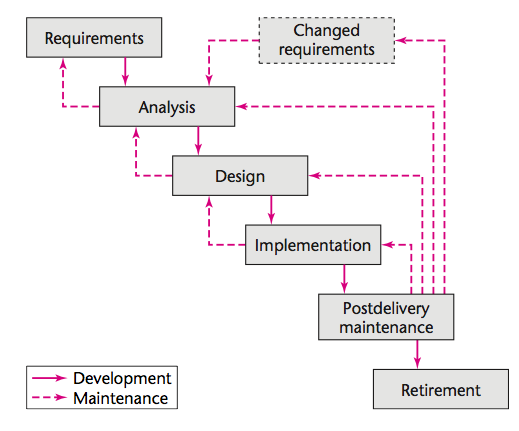
\includegraphics[width=1\textwidth]{waterfall.png}
					\caption{The Waterfall Method}
				\end{figure}
				\item \textbf{Rapid Prototype Model} - Construction of a functional subset of the desired product in order to allow the client and developer to interact
				\begin{figure}
					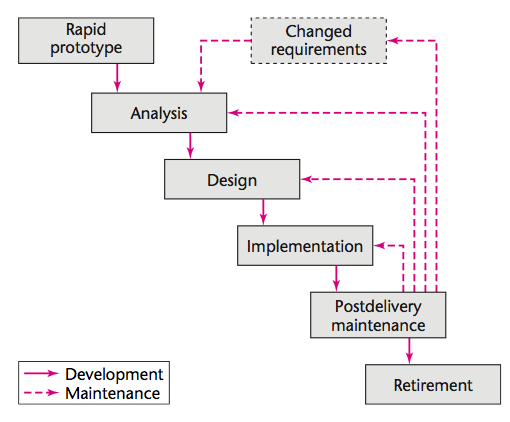
\includegraphics[width=1\textwidth]{rapidPrototype.png}
					\caption{The Rapid Prototype Method}
				\end{figure}
				\item \textbf{Incremental Build Model} - Software is implemented, integrated, and tested as a series of incremental builds
					\begin{itemize}
						\item \textbf{Incremental Build} - Code piece providing a specific function
					\end{itemize}
				\item \textbf{Spiral Model} - A variation of the Waterfall Method in which each phase is preceded by risk analysis in an attempt to control risk
				\begin{figure}
					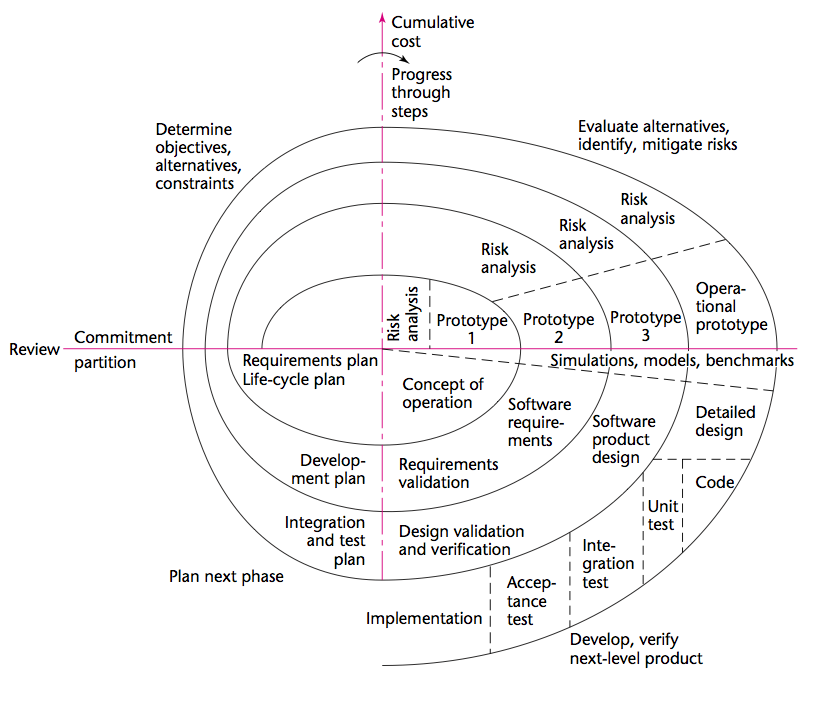
\includegraphics[width=1\textwidth]{spiral.png}
					\caption{The Spiral Model}
				\end{figure}
			\end{itemize}
		\item \textbf{Teams}
			\begin{itemize}
				\item \textbf{Team} - Group of professionals organized in order to complete the task of creating a large software project
				\item \textbf{Jelled Team} - Group of people who are so tightly knit that the attitude is that the whole is greater than the sum of the parts
				\item \textbf{Team Roles}
					\begin{itemize}
						\item \textbf{Team Leader} - Responsible for overseeing all aspects of the team project, holds the tie-breaking vote
						\item \textbf{Technical Lead} - Expert on all technical aspects of the project, in particular the hardware and software used for development
						\item \textbf{Designer} - Designs the project and breaks the project into smaller pieces (modules) for the programmers
						\item \textbf{Lead Programmer} - needs to have an understanding of the project as a whole; organizes all of the other programmers
						\item \textbf{Technical Writer} - Writes all documentation for the project
						\item \textbf{Configuration Management} - Maintains the code base for the project, could include CVS responsibilities
						\item \textbf{Quality Assurance (SQA)} - Writes, maintains, and conducts all testing associated with the project
					\end{itemize}
			\end{itemize}
		\item \textbf{Stepwise Refinement} - Process whereby a project is successively decomposed into more detailed instructions
		\item \textbf{Divide-and-Conquer} - Break a large problem into smaller subproblems that should be easier to solve
		\item \textbf{Separation of Concerns} - Process of breaking a software project into components which overlap as little as possible in relationship to functionality
		\item \textbf{CASE Tools} - Computer-Aided Software Engineering
			\begin{itemize}
				\item \textbf{UpperCASE} - Front end; used in requirements, analysis, and design workflows
				\item \textbf{LowerCASE} - Back end; used in implementation and maintenance activities
				\item \textbf{Data Dictionary} - Computerized list of all data defined within the product (Type and location defined)
				\item \textbf{Consistency Checker} - Tool which checks that everything in the design is in the spec doc and everything in the spec doc is in the design
				\item \textbf{Report Generator} - Tool which generates the code necessary for producing a report (Memory Dumps, etc. ?)
				\item \textbf{Screen Generator} - Tool which generates the code necessary for a data capture screen
				\item \textbf{Structured Editor} - Text editor designed to understand the structure of a program in a programming language, aiding in syntax fault prevention or early detection
				\item \textbf{"Pretty Printer"/Formatter} - Code often included with the structured editor which makes use of the language syntax structure to display the code in a standard manner (Indenting, syntax highlighting, etc.)
				\item \textbf{On-Line Interface Checker} - Editor knows every subprogram declared within the product and its parameter lists
				\item \textbf{OS Front End} - Tool which allows the programmer to give commands to the OS from within the editor
				\item \textbf{Source Level Debugger}
				\item \textbf{Interactive Source Level Debugger}
				\item \textbf{Version Control Tool} - Keeps detailed record of each version of the project
				\item \textbf{Configuration Control Tool} - Manages multiple variations
			\end{itemize}
		\item \textbf{Configuration} - Specific version of each artifact from which a given version of the complete product is built
		\item \textbf{Verification} - Determining whether a phase has been correctly carried out (Takes place at the end of the phase)
		\item \textbf{Validation} - Testing just before a product is delivered to a client to determine if it satisfies the specifications
		\item \textbf{Inception Phase} - Determine whether it is worthwhile to develop the target product
		\item \textbf{Elaboration Phase} - Refine the requirements and architecture, monitor the risks, refine the business case, and produce the Software Project Management Plan (SPMP)
		\item \textbf{Construction Phase} - Produce the first operation-quality version of the product (Beta Release)
		\item \textbf{Transition Phase} - Aim is to ensure that the client's requirements have been met
		\item \textbf{Defects}
			\begin{itemize}
				\item \textbf{Fault} - Human mistake created in software
				\item \textbf{Failure} - Observed incorrect behavior due to a fault
				\item \textbf{Error} - Amount by which a result is incorrect
				\item \textbf{Defect} - Generic term which encompasses Fault, Failure, and Error
			\end{itemize}
		\item \textbf{Software Quality} - Extent to which the product satisfies its expectations
		\item \textbf{Participant Driven Walkthrough} - Members present lists of things they do not understand and things they think are incorrect to the team that is creating the document that is being tested. The team responds to each item.
		\item \textbf{Document Driven Walkthrough} - Chair walks the members through the document with stops at the unclear points or possible faults
		\item \textbf{Inspections}
			\begin{itemize}
				\item \textbf{Overview} - Presentation by one individual responsible for producing it, after which it is given to the participants
				\item \textbf{Preparation} - Participants try to understand the documents using lists of fault types and create checklists
				\item \textbf{Inspection} - One participant walks through, using the checklists, while the moderator creates the written report
				\item \textbf{Rework} - Using the written report of faults, the team resolves the faults
				\item \textbf{Follow-up} - The moderator makes sure that everything in the report has been corrected or addressed and that no new faults were created in repairing the original faults.
			\end{itemize}
		\item \textbf{Inspection Rate} - Number of pages inspected per hour (for specifications and designs) or LOC/hr (for code inspection)
		\item \textbf{Fault Density} - Number of faults per page or per KLOC
		\item \textbf{Fault Detection Rate} - Number of major and minor faults detected per hour
		\item \textbf{Fault Detection Efficiency} - Number of major and minor faults detected per person-hour
		\item \textbf{Unit Testing} - Earliest types of testing, testing the parts of the application (functions, modules, module combinations)
		\item \textbf{Integration Testing} - Validates the overall functionality of each stage
		\item \textbf{Acceptance Testing} - Validates the final product
		\item \textbf{Black Box Test} - Checking correct output for given input as specified by the requirements
		\item \textbf{White Box Test} - Design test to cover all paths through the application
		\item \textbf{Gray Box Test} - Consider limited details of the application with some of the black box techniques
		\item \textbf{Equivalence Partitioning} - Division of the test input data into subsets
		\item \textbf{Boundary Value Analysis} - Testing for values which separate acceptable and unacceptable ranges
		\item \textbf{Statement Coverage} - Every statement should be executed by at least one test
		\item \textbf{Decision Coverage} - Every brand of decision statements is executed by at least one test
		\item \textbf{Utility} - How useful it is or how it meets the needs of the user
		\item \textbf{Reliability} - Measure the mean time between failures; reliable software rarely fails
		\item \textbf{Robustness} - Valid output for valid input, error conditions handled correctly (satisfying the specifications)
		\item \textbf{Performance} - How well it meets constraints
		\item \textbf{Correctness} - Valid output for valid input
		\item \textbf{Module} - Lexically contiguous sequence of statements bounded by boundary symbols, having an associated name
		\item \textbf{Cohesion} - Degree of interaction within a module
			\begin{itemize}
				\item \textbf{Coincidental} - No meaningful relationships among the elements of an entity
				\item \textbf{Logical} - Performs a series of related actions, one of which is selected by the calling module
				\item \textbf{Classical or Temporal} - Performs a series of related actions related over time
				\item \textbf{Procedural} - Performs a series of actions related by the sequence of steps to be followed by the product
				\item \textbf{Communicational} - Performs a series of actions related by the sequence of steps to be followed by the product performed on the same data (Passing the same value to each function in Procedural Cohesion)
				\item \textbf{Information} - Performs multiple functions, each with its own entry point and independent code for each action, all performed on the same data structure
				\item \textbf{Functional} - Performs a single function or action
			\end{itemize}
		\item \textbf{Coupling} - Degree of interaction between two modules
			\begin{itemize}
				\item \textbf{Content} - Software entity references the contents of another entity
				\item \textbf{Common} - Software entities reference a shared global data structure
				\item \textbf{External} - Software entities reference the same externally declared symbol
				\item \textbf{Control} - One entity passes control elements as arguments to another entity
				\item \textbf{Stamp} - A data structure is passed but not entirely used
				\item \textbf{Data} - One entity calls another and are not coupled as described above
			\end{itemize}
		\item  \textbf{Abstraction} - A means of achieving stepwise refinement by suppressing unnecessary details and accentuating relevant details
		\item \textbf{Data Abstraction} - Data structure along with the actions or operations to be performed on that structure
		\item \textbf{Procedural Abstraction} - Conceptualizing in terms of giving a name to a set of high-level actions which are specified by the body of the procedure
		\item \textbf{Information Hiding} - Hiding the implementation details of a module from another using it
		\item \textbf{Abstract Data Type} - Specification of a data type along with the operations on that type
		\item \textbf{Reuse} - Taking components of one product to be used in a different product with different functionality
			\begin{itemize}
				\item \textbf{Accidental/Opportunistic Reuse} - Developers realize that a component from a previous project can be used in a current project
				\item \textbf{Deliberate/Systematic Reuse} - Components are constructed with the intent that they will be reusable
			\end{itemize}
		\item \textbf{Portability} - Software which is significantly easier to modify to run on another platform than it is to recode from scratch
		\item \textbf{Internal Cost} - Cost to the developer to develop the product
		\item \textbf{External Cost} - Cost to the client
		\item \textbf{File} - Collection of logically or physically related records permanently resident in the product (Transaction and Temporary files don't count here)
		\item \textbf{Flow} - Data interface between the product and the environment (screen of report)
		\item \textbf{Process} - Functionally defined logical or arithmetic manipulation of the data (Sorting, validating, updating, etc.)
		\item \textbf{Function Point} - Used to assess the size of the project
		\item \textbf{Product Metrics} - Measure some aspect of the product itself, such as its size or reliability
		\item \textbf{Process Metrics} - Used by the developers to deduce information about the software process
		\item \textbf{Component Reuse} - Element may be used by another program's element
	\end{itemize}
% -----------------------------------------------------------------------------------
\part{Useful Information}
	\chapter{Test 1}
		\section{Draw and Discuss}
			\begin{itemize}
				\item Waterfall Method 
				\item Life-Cycle Model
			\end{itemize}
		\section{Definitions}
			\begin{itemize}
				\item Traceability
				\item Cohesion
				\item Coupling
			\end{itemize}
		\section{Things to Know}
			\begin{itemize}
				\item Advantages and Disadvantages of the Waterfall Method (Section 2.1.1)
				\item Given a project situation, recommend a life-cycle model to use
				\item Project factors related to programming team structure (Section 3.1)
				\item Comparison of walkthroughs and inspections (Section 6.1.2)
				\item Cohesion (Section 7.1.1)
				\item Coupling (Section 7.1.2)
				\item Advantages and Disadvantages of Deliberate Reuse (Section 2.0.4 8.1)
				\item Project Function and Activity (Section 9.3.1)
			\end{itemize}

	\chapter{Agile Presentations}
		\section{Kanban}
			\textit{Ankur Patel}
			\begin{itemize}
				\item Japanese for 'Visual Card'
				\item David Anderson, 2004-2007
				\item Kanban method was originally created by Taiichi Onho in the late 1940s.
				\item Implement business concept of JIT at TPS\\
					\textit{Anderson adapted it to software}
				\item Lots of whiteboards, sticky notes, and sections of each software dev cycle to increase visibility of workflow.
				\item Columns and subcolumns
					\begin{itemize}
						\item Columns for phases
						\item Subcolumns for 'To-Do', 'Doing', 'Done'
					\end{itemize}
				\item Bottlenecks the team's efforts.
				\item Flexible
			\end{itemize}
		\section{Agile Scaling Model}
			\textit{Cody Herring}
			\begin{itemize}
				\item Way of beginning the software development process.
				\item Scott Ambler
				\item Three Categories
					\begin{itemize}
						\item Core Agile Development
							\begin{itemize}
								\item Beginning role in the development cycle
							\end{itemize}
						\item Agile Delivery
							\begin{itemize}
								\item Repeatable results with just the right amount of ceremony for the situations they face.
							\end{itemize}
						\item Agile at Scale
					\end{itemize}
				\item First step to take
					\begin{itemize}
						\item Adopt disciplined agile delivery life cycle
					\end{itemize}
				\item Complementary strategy to other methodologies
			\end{itemize}
		\section{Agile Software Development}
			\textit{Jared Cox}
			\begin{itemize}
				\item James Highsmith and Sam Bayer
				\item Came from RSD
					\begin{itemize}
						\item Like RSD, but more iterative
					\end{itemize}
				\item Six Characteristics
					\begin{itemize}
						\item Mission-driven
						\item Component-based
						\item Iterative
						\item Time-boxing
						\item Risk-driven
						\item Change-tolerant
					\end{itemize}
				\item Three Step Life Cycle
					\begin{itemize}
						\item Speculate
						\item Collaborate
						\item Learn
					\end{itemize}
			\end{itemize}
		\section{Crystal Methods}
			\textit{James Reatherford}
			\begin{itemize}
				\item Alistair Cockburn
				\item Series of related methods for projects of various size and complexity
				\item Incremental
				\item Real crystals have two main properties: color and hardness
				\begin{itemize}
					\item Color - size of team
					\item Hardness - complexity of the project in terms of cost of failure
				\end{itemize}
				\item Very much like agile manifesto
			\end{itemize}
		\section{Crystal Clear}
			\textit{Ashutosh Karki}
			\begin{itemize}
				\item Lowest hardness of Crystal Family
				\item Osmotic communication
				\item Optimized
			\end{itemize}
		\section{Agile Modeling}
			\textit{CJ Stokes}
			\begin{itemize}
				\item Scott Ambler
				\item Values
					\begin{itemize}
						\item Communication
						\item Simplicity
						\item Feedback
						\item Courage
						\item Humility
					\end{itemize}
				\item Principles
					\begin{itemize}
						\item Software is primary
						\item Enabling the next effort is secondary
						\item Travel light
						\item Assume simplicity
						\item Embrace change
						\item Incremental change
						\item Model with a purpose
						\item Multiple models
						\item Quality work
						\item Rapid feedback
					\end{itemize}
				\item Practices
					\begin{itemize}
						\item Iterative and Incremental Modeling
						\item Teamwork
					\end{itemize}
			\end{itemize}
		\section{Extreme Programming}
			\subsection{Phillip Clark}
				\begin{itemize}
					\item Kent Beck
					\item Heavily based on test-driven development and iterative and incremental development
					\item Takes common sense principles to an extreme level
					\item Coding is the key activity.
					\item System architecture is not documented (The code is the documentation)
					\item Four values
						\begin{enumerate}
							\item Communication
							\item Simplicity
								\begin{itemize}
									\item "Live for today"
								\end{itemize}
							\item Feedback
								\begin{itemize}
									\item "Learning to drive"
								\end{itemize}
							\item Courage
						\end{enumerate}
					\item Twelve Core Practices
						\begin{enumerate}
							\item The Planning Game
							\item Small releases
							\item Metaphor
							\item Simple design
							\item Testing
							\item Refactoring
							\item Pair programming
							\item Collective ownership
							\item Continuous integration
							\item 40-hour week
								\begin{itemize}
									\item Not allowed to work overtime two weeks in a row.
								\end{itemize}
							\item On-site customer
							\item Coding standards
						\end{enumerate}
					\item Cool features
						\begin{itemize}
							\item Food
							\item Parties after releases
							\item Interesting office arrangement
							\item No documentation
						\end{itemize}
				\end{itemize}
			\subsection{Michael Debs}
				\begin{itemize}
					\item Working software over comprehensive documentation
					\item Responding to change over following a plan
					\item Simplicity
					\item Refactoring
					\item Pair programming
					\item Collective ownership
						\begin{itemize}
							\item Trust
						\end{itemize}
					\item Small Development teams
				\end{itemize}
		\section{DSDM}
			\textit{Patrick Lindsay}
		\section{Scrum}
			\textit{Atticus Wright}
			\begin{itemize}
				\item Four main tenets
					\begin{itemize}
						\item Individuals and interactions over precesses and tools
							\begin{itemize}
								\item Scrum dev teams are self-organizing and rely heavily on communication
								\item Daily scrums
							\end{itemize}
						\item Working software over documentation
							\begin{itemize}
								\item The goal of each sprint is to have developed functionality for a project that could be released to the public
							\end{itemize}
						\item Customer collaboration over contract negotiation
							\begin{itemize}
								\item Product owner works with stakeholders
							\end{itemize}
					\end{itemize}
				\item Works well in chaotic, changing environments
				\item Produces working software early and often
				\item Features with high priorities are first
				\item Catch and fix problem quickly
				\item Increases morale and productivity
				\item Supports knowledge sharing
				\item May be a wrapper for other methods
				\\
				\item Weaknesses
					\begin{itemize}
						\item Can result in inadequate documentation with too much information inside team members' minds
						\item Teams may try to modify Scrum to prevent failure
						\item Not great for novices
						\item May prevent formation of long-term goals
						\item Not suitable for teams of more than 10 people
					\end{itemize}
				\item Sped up, less structured spiral model
				\item Incremental
				\item Lots of scrum in lots of places
			\end{itemize}
		\section{Enterprise Agile}
			\textit{Alla Salah}
			\begin{itemize}
				\item Created by Mike Beedle in 1999
				\item Hybrid of Scrum and XP
				\item Mainly used in organizations with really big projects
				\item Can operate in concurrent multi-project environment
				\item Emphasizes project reusability
				\item Features from scrum form its management structure
				\item Some of XP's features for the actual development process
				\item Daily scrum meetings, scrum master, sprint backlogs
				\item Pair programming, refactoring, product owner
				\item Four main phases
					\begin{itemize}
						\item Planning - sprint backlog and overall project organization
						\item Designing - constructing the class and object diagram
						\item Coding - pair programming and refactoring
						\item Testing - validation
					\end{itemize}
				\item Advantages
					\begin{itemize}
						\item Eventually develop large repository of reusable models
						\item Scalable for project size and complexity
					\end{itemize}
				\item Disadvantages
					\begin{itemize}
						\item Reusable code is expensive
						\item Requires competent team members
					\end{itemize}
			\end{itemize}
		\section{Feature Driven Development}
			\textit{Hong Bin Yu}
			\begin{itemize}
				\item First proposed by Peter Coad.
				\item Agile, highly adaptive software development process
					\begin{itemize}
						\item Has lots of short term iteration
						\item Quality is concerned at all steps
						\item Delivers frequent client-valued results at all steps
						\item Reports accurate significant changes
					\end{itemize}
				\item Five Phases
					\begin{enumerate}
						\item Develop an overall model
						\item Build a feature list
						\item Plan by feature
						\item Design by feature
						\item Build by feature
					\end{enumerate}
				\item Eight Practices
					\begin{enumerate}
						\item Domain object modeling
						\item Developing by feature
						\item Class (code) ownership
							\begin{itemize}
								\item "Everybody gets one." - Every developer is an expert on one part of the project
							\end{itemize}
						\item Feature teams
						\item Inspection
						\item Regular build schedule
						\item Configuration management
						\item Reporting/Visibility of results
					\end{enumerate}
				\item Has a mathematical formula for project progress
			\end{itemize}
		\section{Pragmatic Programming}
			\textit{Ricky Moore}
			\begin{itemize}
				\item Not so well defined
				\item Main point is to prevent problems
				\item Invented by Andrew Hunt and David Thomas - \textit{The Pragmatic Programmer}
				\item Techniques are complimentary to other agile methods
			\end{itemize}
		\section{Internet-Speed Development Method}
			\textit{Elisabeth McClellan}
			\begin{itemize}
				\item Quick and dirty
				\item Main idea is to beat your competitors to the punch
				\item Similar to code-and-fix
				\item Doesn't concern itself with maintenance; procrastinates debugging
				\item Love code reuse
				\item Stable architecture is suggested, but not mandatory
			\end{itemize}
		\section{Lean Software Development}
			\textit{Jordan Shook}
			\begin{itemize}
				\item Mary and Tom Poppendieck - 2003
				\item Seven Principles
					\begin{enumerate}
						\item Eliminate Waste
						\item Amplify Learning
						\item Decide as late as possible
						\item Deliver as fast as possible
						\item Empower the team
						\item Build integrity into the code
						\item See the whole
					\end{enumerate}
				\item No unnecessary documentation
				\item Can allow creativity, but that can be a bad thing
			\end{itemize}
		\section{Agile Unified Process}
			\textit{Jason Smith}
			\begin{itemize}
				\item Scott Ambler - 2005
				\item Simple easy to understand approach to business software using Agile principles
				\item Nature
					\begin{itemize}
						\item Inception
						\item Elaboration
						\item Construction
						\item Transition
					\end{itemize}
				\item Philosophies
					\begin{enumerate}
						\item Staff needs to know what they are doing
						\item Simplicity
						\item Agility
						\item Focus on high-level activities
						\item Tool independence
						\item You'll want to tailor this product to meet your own needs
					\end{enumerate}
				\item Best Practices
					\begin{itemize}
						\item Sign off artifacts
						\item Need-based artifacts
						\item Discuss, visualize and write
						\item Single repository
						\item Requirement prioritization
						\item Requirement envisioning
						\item Executable specifications
						\item Model storming
						\item Model in advance
						\item Multiple models
						\item Effective communication
						\item Accept change
					\end{itemize}
				\item Delivery over time
			\end{itemize}
		\section{Graphical System Design}
			\textit{Pengcheng Zhao}
			\begin{itemize}
				\item The process of defining and developing the hardware and software architecture, components, modules, and system
				\item Goal is to satisfy requirements with a graphical programming language
				\item Mainly used to develop embedded systems
				\item Problem - software engineers are usually short on knowledge about specific hardwares, but hardware experts can't completely understand algorithmic software development
				\item Both parts can use the same tools (LabVIEW)
				\item The team size can be two or more
				\item Save time and money
			\end{itemize}
\end{document}